\mysection{ARM}
\myindex{ARM}

\subsection{Terminology}

ARM was initially developed as 32-bit \ac{CPU}, 
so that's why a \emph{word} here, unlike x86, is 32-bit.

\begin{description}
	\item[byte] 8-bit.
		The DB assembly directive is used for defining variables and arrays of bytes.
	\item[halfword] 16-bit. DCW assembly directive \dittoclosing.
	\item[word] 32-bit.  DCD assembly directive \dittoclosing.
	\item[doubleword] 64-bit.
	\item[quadword] 128-bit.
\end{description}

\subsection{Versions}

\begin{itemize}
\item ARMv4: Thumb mode introduced.

\item ARMv6: used in iPhone 1st gen., iPhone 3G (Samsung 32-bit RISC ARM 1176JZ(F)-S that supports Thumb-2)

\item ARMv7: Thumb-2 was added (2003).
was used in iPhone 3GS, iPhone 4, iPad 1st gen. (ARM Cortex-A8), iPad 2 (Cortex-A9),
iPad 3rd gen.

\item ARMv7s: New instructions added.
iPhone 5, iPhone 5c, iPad 4th gen. (Apple A6).

\item ARMv8: 64-bit CPU, \ac{AKA} ARM64 \ac{AKA} AArch64.
Was used in iPhone 5S, iPad Air (Apple A7).
There is no Thumb mode in 64-bit mode, only ARM (4-byte instructions).
\end{itemize}

% sections
\subsection{General purpose registers}

It is possible to access many registers by byte or 16-bit word parts.

It is all inheritance from older Intel CPUs (up to the 8-bit 8080) 
still supported for backward compatibility.
Older 8-bit CPUs (8080) had 16-bit registers divided by two.

Programs written for 8080 could access the low byte part of 16-bit registers, high byte part
or the whole 16-bit register.

Perhaps, this feature was left in 8086 as a helper for easier porting.

This feature is usually not present in \ac{RISC} CPUs.

\myindex{x86-64}
Registers prefixed with \TT{R-} appeared in x86-64, and those prefixed with \TT{E-}---in 80386.

Thus, R-registers are 64-bit, and E-registers---32-bit.

8 more \ac{GPR}'s were added in x86-86: R8-R15.

N.B.: 
In the Intel manuals the byte parts of these registers are prefixed by \emph{L}, e.g.: \emph{R8L}, but \ac{IDA}
names these registers by adding the \emph{B} suffix, e.g.: \emph{R8B}.

\subsubsection{RAX/EAX/AX/AL}
\RegTableOne{RAX}{EAX}{AX}{AH}{AL}

\ac{AKA} accumulator.
The result of a function is usually returned via this register.

\subsubsection{RBX/EBX/BX/BL}
\RegTableOne{RBX}{EBX}{BX}{BH}{BL}

\subsubsection{RCX/ECX/CX/CL}
\RegTableOne{RCX}{ECX}{CX}{CH}{CL}

\ac{AKA} counter:
in this role it is used in REP prefixed instructions and also in shift instructions
(SHL/SHR/RxL/RxR).

\subsubsection{RDX/EDX/DX/DL}
\RegTableOne{RDX}{EDX}{DX}{DH}{DL}

\subsubsection{RSI/ESI/SI/SIL}
\RegTableTwo{RSI}{ESI}{SI}{SIL}

\ac{AKA} \q{source index}. Used as source in the instructions
REP MOVSx, REP CMPSx.

\subsubsection{RDI/EDI/DI/DIL}
\RegTableTwo{RDI}{EDI}{DI}{DIL}

\ac{AKA} \q{destination index}.
Used as a pointer to the destination in the instructions
REP MOVSx, REP STOSx.

% TODO навести тут порядок
\subsubsection{R8/R8D/R8W/R8L}
\RegTableFour{R8}{R8D}{R8W}{R8L}

\subsubsection{R9/R9D/R9W/R9L}
\RegTableFour{R9}{R9D}{R9W}{R9L}

\subsubsection{R10/R10D/R10W/R10L}
\RegTableFour{R10}{R10D}{R10W}{R10L}

\subsubsection{R11/R11D/R11W/R11L}
\RegTableFour{R11}{R11D}{R11W}{R11L}

\subsubsection{R12/R12D/R12W/R12L}
\RegTableFour{R12}{R12D}{R12W}{R12L}

\subsubsection{R13/R13D/R13W/R13L}
\RegTableFour{R13}{R13D}{R13W}{R13L}

\subsubsection{R14/R14D/R14W/R14L}
\RegTableFour{R14}{R14D}{R14W}{R14L}

\subsubsection{R15/R15D/R15W/R15L}
\RegTableFour{R15}{R15D}{R15W}{R15L}

\subsubsection{RSP/ESP/SP/SPL}
\RegTableFour{RSP}{ESP}{SP}{SPL}

\ac{AKA} \gls{stack pointer}. 
Usually points to the current stack except in those cases when it is not yet initialized.

\subsubsection{RBP/EBP/BP/BPL}
\RegTableFour{RBP}{EBP}{BP}{BPL}

\ac{AKA} frame pointer. 
Usually used for local variables and accessing the arguments of the function. More about it: (\myref{stack_frame}).

\subsubsection{RIP/EIP/IP}

\begin{center}
\begin{tabular}{ | l | l | l | l | l | l | l | l | l |}
\hline
\RegHeaderTop \\
\hline
\RegHeader \\
\hline
\multicolumn{8}{ | c | }{RIP\textsuperscript{x64}} \\
\hline
\multicolumn{4}{ | c | }{} & \multicolumn{4}{ c | }{EIP} \\
\hline
\multicolumn{6}{ | c | }{} & \multicolumn{2}{ c | }{IP} \\
\hline
\end{tabular}
\end{center}

\ac{AKA} \q{instruction pointer}
\footnote{Sometimes also called \q{program counter}}.
Usually always points to the instruction to be executed right now.
Cannot be modified, however, it is possible to do this (which is equivalent):

\begin{lstlisting}
MOV EAX, ...
JMP EAX
\end{lstlisting}

Or:

\begin{lstlisting}
PUSH value
RET
\end{lstlisting}

\subsubsection{CS/DS/ES/SS/FS/GS}

16-bit registers containing code selector (CS), 
data selector (DS), stack selector (SS).\\
\\
\myindex{TLS}
\myindex{Windows!TIB}
FS in win32 points to \ac{TLS}, GS took this role in Linux.
It is made so for faster access to the \ac{TLS} and other structures like the \ac{TIB}.
\\
In the past, these registers were used as segment registers (\myref{8086_memory_model}).

\subsubsection{Flags register}
\myindex{x86!\Registers!\Flags}
\label{EFLAGS}
\ac{AKA} EFLAGS.

\small
\begin{center}
\begin{tabular}{ | l | l | l | }
\hline
\headercolor{} Bit (mask) &
\headercolor{} Abbreviation (meaning) &
\headercolor{} Description \\
\hline
0 (1) & CF (Carry) & The CLC/STC/CMC instructions are used \\
      &            & for setting/resetting/toggling this flag \\
\hline
2 (4) & PF (Parity) & (\myref{parity_flag}). \\
\hline
4 (0x10) & AF (Adjust) & Exist solely for work with \ac{BCD}-numbers \\
\hline
6 (0x40) & ZF (Zero) & Setting to 0 \\
         &           & if the last operation's result is equal to 0. \\
\hline
7 (0x80) & SF (Sign) &  \\
\hline
8 (0x100) & TF (Trap) & Used for debugging. \\
&         &             If turned on, an exception is to be \\
&         &             generated after each instruction's execution. \\
\hline
9 (0x200) & IF (Interrupt enable) & Are interrupts enabled. \\
          &                       & The CLI/STI instructions are used \\
	  &                       & for setting/resetting the flag \\
\hline
10 (0x400) & DF (Direction) & A direction is set for the \\
           &                & REP MOVSx/CMPSx/LODSx/SCASx instructions.\\
           &                & The CLD/STD instructions are used \\
	   &                & for setting/resetting the flag \\
	   &                & See also: \myref{memmove_and_DF}. \\
\hline
11 (0x800) & OF (Overflow) & Overflow flag \\
\hline
12, 13 (0x3000) & IOPL (I/O privilege level)\textsuperscript{i286} & \\
\hline
14 (0x4000) & NT (Nested task)\textsuperscript{i286} & \\
\hline
16 (0x10000) & RF (Resume)\textsuperscript{i386} & Used for debugging. \\
             &                  & The CPU ignores the hardware \\
	     &                  & breakpoint in DRx if the flag is set. \\
\hline
17 (0x20000) & VM (Virtual 8086 mode)\textsuperscript{i386} & \\
\hline
18 (0x40000) & AC (Alignment check)\textsuperscript{i486} & \\
\hline
19 (0x80000) & VIF (Virtual interrupt)\textsuperscript{i586} & \\
\hline
20 (0x100000) & VIP (Virtual interrupt pending)\textsuperscript{i586} & \\
\hline
21 (0x200000) & ID (Identification)\textsuperscript{i586} & \\
\hline
\end{tabular}
\end{center}
\normalsize

All the rest flags are reserved.

\subsection{FPU registers}

\myindex{x86!FPU}
8 80-bit registers working as a stack: ST(0)-ST(7).
N.B.: \ac{IDA} calls ST(0) as just ST.
Numbers are stored in the IEEE 754 format.

\emph{long double} value format:

\bigskip
% a hack used here! http://tex.stackexchange.com/questions/73524/bytefield-package
\begin{center}
\begingroup
\makeatletter
\let\saved@bf@bitformatting\bf@bitformatting
\renewcommand*{\bf@bitformatting}{%
	\ifnum\value{header@val}=21 %
	\value{header@val}=62 %
	\else\ifnum\value{header@val}=22 %
	\value{header@val}=63 %
	\else\ifnum\value{header@val}=23 %
	\value{header@val}=64 %
	\else\ifnum\value{header@val}=30 %
	\value{header@val}=78 %
	\else\ifnum\value{header@val}=31 %
	\value{header@val}=79 %
	\fi\fi\fi\fi\fi
	\saved@bf@bitformatting
}%
\begin{bytefield}[bitwidth=0.03\linewidth]{32}
	\bitheader[endianness=big]{0,21,22,23,30,31} \\
	\bitbox{1}{S} &
	\bitbox{8}{exponent} &
	\bitbox{1}{I} &
	\bitbox{22}{mantissa or fraction}
\end{bytefield}
\endgroup
\end{center}

\begin{center}
( S --- sign, I --- integer part )
\end{center}

\label{FPU_control_word}
\subsubsection{Control Word}

Register controlling the behavior of the \ac{FPU}.

%\small
\begin{center}
\begin{tabular}{ | l | l | l | }
\hline
Bit &
Abbreviation (meaning) &
Description \\
\hline
0   & IM (Invalid operation Mask) & \\
\hline
1   & DM (Denormalized operand Mask) & \\
\hline
2   & ZM (Zero divide Mask) & \\
\hline
3   & OM (Overflow Mask) & \\
\hline
4   & UM (Underflow Mask) & \\
\hline
5   & PM (Precision Mask) & \\
\hline
7   & IEM (Interrupt Enable Mask) & Exceptions enabling, 1 by default (disabled) \\
\hline
8, 9 & PC (Precision Control) &  \\
     &                        & 00 ~--- 24 bits (REAL4) \\
     &                        & 10 ~--- 53 bits (REAL8) \\
     &                        & 11 ~--- 64 bits (REAL10) \\
\hline
10, 11 & RC (Rounding Control) &  \\
       &                       & 00 ~--- (by default) round to nearest \\
       &                       & 01 ~--- round toward $-\infty$ \\
       &                       & 10 ~--- round toward $+\infty$ \\
       &                       & 11 ~--- round toward 0 \\
\hline
12 & IC (Infinity Control) & 0 ~--- (by default) treat $+\infty$ and $-\infty$ as unsigned \\
   &                       & 1 ~--- respect both $+\infty$ and $-\infty$ \\
\hline
\end{tabular}
\end{center}
%\normalsize

The PM, UM, OM, ZM, DM, IM 
flags define if to generate exception in the case of a corresponding error.

\subsubsection{Status Word}

\label{FPU_status_word}
Read-only register.

\small
\begin{center}
\begin{tabular}{ | l | l | l | }
\hline
Bit &
Abbreviation (meaning) &
Description \\
\hline
15   & B (Busy) & Is FPU do something (1)
or results are ready (0) \\
\hline
14   & C3 & \\
\hline
13, 12, 11 & TOP & points to the currently zeroth register \\
\hline
10 & C2 & \\
\hline
9  & C1 & \\
\hline
8  & C0 & \\
\hline
7  & IR (Interrupt Request) & \\
\hline
6  & SF (Stack Fault) & \\
\hline
5  & P (Precision) & \\
\hline
4  & U (Underflow) & \\
\hline
3  & O (Overflow) & \\
\hline
2  & Z (Zero) & \\
\hline
1  & D (Denormalized) & \\
\hline
0  & I (Invalid operation) & \\
\hline
\end{tabular}
\end{center}
\normalsize

The SF, P, U, O, Z, D, I bits signal about exceptions.

About the C3, C2, C1, C0 you can read more here: (\myref{Czero_etc}).

N.B.: When ST(x) is used, the FPU adds $x$ to TOP (by modulo 8) and that is how it gets 
the internal register's number.

\subsubsection{Tag Word}

The register has current information about the usage of numbers registers.

\begin{center}
\begin{tabular}{ | l | l | l | }
\hline
Bit & Abbreviation (meaning) \\
\hline
15, 14 & Tag(7) \\
\hline
13, 12 & Tag(6) \\
\hline
11, 10 & Tag(5) \\
\hline
9, 8 & Tag(4) \\
\hline
7, 6 & Tag(3) \\
\hline
5, 4 & Tag(2) \\
\hline
3, 2 & Tag(1) \\
\hline
1, 0 & Tag(0) \\
\hline
\end{tabular}
\end{center}

Each tag contains information about a physical FPU register (R(x)), not logical (ST(x)).

For each tag:

\begin{itemize}
\item 00 ~--- The register contains a non-zero value
\item 01 ~--- The register contains 0
\item 10 ~--- The register contains a special value (\ac{NAN}, $\infty$, or denormal)
\item 11 ~--- The register is empty
\end{itemize}

\subsection{SIMD registers}

\subsubsection{MMX registers}

8 64-bit registers: MM0..MM7.

\subsubsection{SSE and AVX registers}

\myindex{x86-64}
SSE: 8 128-bit registers: XMM0..XMM7.
In the x86-64 8 more registers were added: XMM8..XMM15.

AVX is the extension of all these registers to 256 bits.

\subsection{Debugging registers}

Used for hardware breakpoints control.

\begin{itemize}
	\item DR0 --- address of breakpoint \#1
	\item DR1 --- address of breakpoint \#2
	\item DR2 --- address of breakpoint \#3
	\item DR3 --- address of breakpoint \#4
	\item DR6 --- a cause of break is reflected here
	\item DR7 --- breakpoint types are set here
\end{itemize}

\subsubsection{DR6}
\myindex{x86!\Registers!DR6}

\begin{center}
\begin{tabular}{ | l | l | }
\hline
\headercolor\ Bit (mask) &
\headercolor\ Description \\
\hline
0 (1)       &  B0 --- breakpoint \#1 has been triggered \\
\hline
1 (2)       &  B1 --- breakpoint \#2 has been triggered \\
\hline
2 (4)       &  B2 --- breakpoint \#3 has been triggered \\
\hline
3 (8)       &  B3 --- breakpoint \#4 has been triggered \\
\hline
13 (0x2000) &  BD --- modification attempt of one of the DRx registers. \\
            &  may be raised if GD is enabled \\
\hline
14 (0x4000) &  BS --- single step breakpoint (TF flag has been set in EFLAGS). \\
	    &  Highest priority. Other bits may also be set. \\
\hline
% TODO: describe BT
15 (0x8000) &  BT (task switch flag) \\
\hline
\end{tabular}
\end{center}

N.B. A single step breakpoint is a breakpoint which occurs after each instruction.
It can be enabled by setting TF in EFLAGS (\myref{EFLAGS}).

\subsubsection{DR7}
\myindex{x86!\Registers!DR7}

Breakpoint types are set here.

%\small
\begin{center}
\begin{tabular}{ | l | l | }
\hline
\headercolor\ Bit (mask) &
\headercolor\ Description \\
\hline
0 (1)       &  L0 --- enable breakpoint \#1 for the current task \\
\hline
1 (2)       &  G0 --- enable breakpoint \#1 for all tasks \\
\hline
2 (4)       &  L1 --- enable breakpoint \#2 for the current task \\
\hline
3 (8)       &  G1 --- enable breakpoint \#2 for all tasks \\
\hline
4 (0x10)    &  L2 --- enable breakpoint \#3 for the current task \\
\hline
5 (0x20)    &  G2 --- enable breakpoint \#3 for all tasks \\
\hline
6 (0x40)    &  L3 --- enable breakpoint \#4 for the current task \\
\hline
7 (0x80)    &  G3 --- enable breakpoint \#4 for all tasks \\
\hline
8 (0x100)   &  LE --- not supported since P6 \\
\hline
9 (0x200)   &  GE --- not supported since P6 \\
\hline
13 (0x2000) &  GD --- exception is to be raised if any MOV instruction \\
            & tries to modify one of the DRx registers \\
\hline
16,17 (0x30000)    &  breakpoint \#1: R/W --- type \\
\hline
18,19 (0xC0000)    &  breakpoint \#1: LEN --- length \\
\hline
20,21 (0x300000)   &  breakpoint \#2: R/W --- type \\
\hline
22,23 (0xC00000)   &  breakpoint \#2: LEN --- length \\
\hline
24,25 (0x3000000)  &  breakpoint \#3: R/W --- type \\
\hline
26,27 (0xC000000)  &  breakpoint \#3: LEN --- length \\
\hline
28,29 (0x30000000) &  breakpoint \#4: R/W --- type \\
\hline
30,31 (0xC0000000) &  breakpoint \#4: LEN --- length \\
\hline
\end{tabular}
\end{center}
%\normalsize

The breakpoint type is to be set as follows (R/W):

\begin{itemize}
\item 00 --- instruction execution
\item 01 --- data writes
\item 10 --- I/O reads or writes (not available in user-mode)
\item 11 --- on data reads or writes
\end{itemize}

N.B.: breakpoint type for data reads is absent, indeed. \\
\\
Breakpoint length is to be set as follows (LEN):

\begin{itemize}
\item 00 --- one-byte
\item 01 --- two-byte
\item 10 --- undefined for 32-bit mode, eight-byte in 64-bit mode
\item 11 --- four-byte
\end{itemize}


% TODO: control registers

\mysection{Finding the right instructions}

If the program is utilizing FPU instructions and there are very few of them in the code,
one can try to check each one manually with a debugger.

\par For example, we may be interested how Microsoft Excel calculates the formulae entered by user.
For example, the division operation.

\myindex{\GrepUsage}
\myindex{x86!\Instructions!FDIV}

If we load excel.exe (from Office 2010) version 14.0.4756.1000 into \IDA, make a full listing
and to find every \FDIV instruction (except the ones which use constants as a second 
operand---obviously, they do not suit us):

\begin{lstlisting}
cat EXCEL.lst | grep fdiv | grep -v dbl_ > EXCEL.fdiv
\end{lstlisting}

\dots then we see that there are 144 of them.

\par We can enter a string like \TT{=(1/3)} in Excel and check each instruction.

\myindex{tracer}

\par By checking each instruction in a debugger or \tracer
(one may check 4 instruction at a time),
we get lucky and the sought-for instruction is just the 14th:

\begin{lstlisting}[style=customasmx86]
.text:3011E919 DC 33          fdiv    qword ptr [ebx]
\end{lstlisting}

\begin{lstlisting}
PID=13944|TID=28744|(0) 0x2f64e919 (Excel.exe!BASE+0x11e919)
EAX=0x02088006 EBX=0x02088018 ECX=0x00000001 EDX=0x00000001
ESI=0x02088000 EDI=0x00544804 EBP=0x0274FA3C ESP=0x0274F9F8
EIP=0x2F64E919
FLAGS=PF IF
FPU ControlWord=IC RC=NEAR PC=64bits PM UM OM ZM DM IM 
FPU StatusWord=
FPU ST(0): 1.000000
\end{lstlisting}

\ST{0} holds the first argument (1) and second one is in \TT{[EBX]}.\\
\\
\myindex{x86!\Instructions!FDIV}

The instruction after \FDIV (\TT{FSTP}) writes the result in memory:\\

\begin{lstlisting}[style=customasmx86]
.text:3011E91B DD 1E          fstp    qword ptr [esi]
\end{lstlisting}

If we set a breakpoint on it, we can see the result:

\begin{lstlisting}
PID=32852|TID=36488|(0) 0x2f40e91b (Excel.exe!BASE+0x11e91b)
EAX=0x00598006 EBX=0x00598018 ECX=0x00000001 EDX=0x00000001
ESI=0x00598000 EDI=0x00294804 EBP=0x026CF93C ESP=0x026CF8F8
EIP=0x2F40E91B
FLAGS=PF IF
FPU ControlWord=IC RC=NEAR PC=64bits PM UM OM ZM DM IM 
FPU StatusWord=C1 P 
FPU ST(0): 0.333333
\end{lstlisting}

Also as a practical joke, we can modify it on the fly:

\begin{lstlisting}
tracer -l:excel.exe bpx=excel.exe!BASE+0x11E91B,set(st0,666)
\end{lstlisting}

\begin{lstlisting}
PID=36540|TID=24056|(0) 0x2f40e91b (Excel.exe!BASE+0x11e91b)
EAX=0x00680006 EBX=0x00680018 ECX=0x00000001 EDX=0x00000001
ESI=0x00680000 EDI=0x00395404 EBP=0x0290FD9C ESP=0x0290FD58
EIP=0x2F40E91B
FLAGS=PF IF
FPU ControlWord=IC RC=NEAR PC=64bits PM UM OM ZM DM IM 
FPU StatusWord=C1 P 
FPU ST(0): 0.333333
Set ST0 register to 666.000000
\end{lstlisting}

Excel shows 666 in the cell, finally convincing us that we have found the right point.

\begin{figure}[H]
\centering
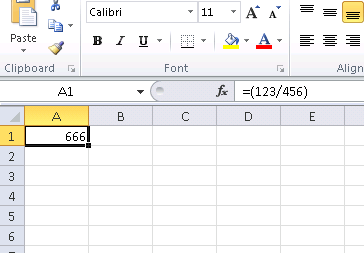
\includegraphics[width=0.6\textwidth]{digging_into_code/Excel_prank.png}
\caption{The practical joke worked}
\end{figure}

If we try the same Excel version, but in x64,
we will find only 12 \FDIV instructions there,
and the one we looking for is the third one.

\begin{lstlisting}
tracer.exe -l:excel.exe bpx=excel.exe!BASE+0x1B7FCC,set(st0,666)
\end{lstlisting}

\myindex{x86!\Instructions!DIVSD}

It seems that a lot of division operations of \Tfloat and \Tdouble types, were replaced by the compiler with SSE instructions
like \TT{DIVSD} (\TT{DIVSD} is present 268 times in total).

